%%%%%%%%%%%%%%%%%%%%%%%%%%%%%%%%%%%%%%%%%
% Beamer Presentation
% LaTeX Template
% Version 1.0 (10/11/12)
%
% This template has been downloaded from:
% http://www.LaTeXTemplates.com
%
% License:
% CC BY-NC-SA 3.0 (http://creativecommons.org/licenses/by-nc-sa/3.0/)
%
%%%%%%%%%%%%%%%%%%%%%%%%%%%%%%%%%%%%%%%%%

%----------------------------------------------------------------------------------------
%	PACKAGES AND THEMES
%----------------------------------------------------------------------------------------

\documentclass{beamer}

\mode<presentation> {

% The Beamer class comes with a number of default slide themes
% which change the colors and layouts of slides. Below this is a list
% of all the themes, uncomment each in turn to see what they look like.

%\usetheme{default}
%\usetheme{AnnArbor}
%\usetheme{Antibes}
%\usetheme{Bergen}
%\usetheme{Berkeley}
%\usetheme{Berlin}
%\usetheme{Boadilla}
%\usetheme{CambridgeUS}
%\usetheme{Copenhagen}
%\usetheme{Darmstadt}
%\usetheme{Dresden}
%\usetheme{Frankfurt}
%\usetheme{Goettingen}
%\usetheme{Hannover}
%\usetheme{Ilmenau}
%\usetheme{JuanLesPins}
%\usetheme{Luebeck}
%\usetheme{Madrid}
%\usetheme{Malmoe}
%\usetheme{Marburg}
%\usetheme{Montpellier}
%\usetheme{PaloAlto}
%\usetheme{Pittsburgh}
%\usetheme{Rochester}
%\usetheme{Singapore}
%\usetheme{Szeged}
%\usetheme{Warsaw}

% As well as themes, the Beamer class has a number of color themes
% for any slide theme. Uncomment each of these in turn to see how it
% changes the colors of your current slide theme.

%\usecolortheme{albatross}
%\usecolortheme{beaver}
%\usecolortheme{beetle}
%\usecolortheme{crane}
%\usecolortheme{dolphin}
%\usecolortheme{dove}
%\usecolortheme{fly}
%\usecolortheme{lily}
%\usecolortheme{orchid}
%\usecolortheme{rose}
%\usecolortheme{seagull}
%\usecolortheme{seahorse}
%\usecolortheme{whale}
%\usecolortheme{wolverine}

%\setbeamertemplate{footline} % To remove the footer line in all slides uncomment this line
%\setbeamertemplate{footline}[page number] % To replace the footer line in all slides with a simple slide count uncomment this line

%\setbeamertemplate{navigation symbols}{} % To remove the navigation symbols from the bottom of all slides uncomment this line
}

\usepackage{graphicx} % Allows including images
\usepackage{booktabs} % Allows the use of \toprule, \midrule and \bottomrule in tables
\usepackage{datetime}

%----------------------------------------------------------------------------------------
%	TITLE PAGE
%----------------------------------------------------------------------------------------

\title[]{Optimising compiler from OCaml to WebAssembly} % The short title appears at the bottom of every slide, the full title is only on the title page

\author{Douglas Boyle} % Your name
\newdate{date}{16}{10}{2019}
\date{\formatdate{11}{2}{2021}} % Date, can be changed to a custom date

\begin{document}

\begin{frame}
\titlepage % Print the title page as the first slide
\end{frame}


%----------------------------------------------------------------------------------------
%	PRESENTATION SLIDES
%----------------------------------------------------------------------------------------

\begin{frame}\frametitle{Overview} 
\includegraphics[scale=0.37]{overview}
\begin{itemize}
\item Compiler for integer and basic floating point operations
\item Benchmark programs in OCaml, Grain and C
\item Compared against Js\_of\_ocaml, Grain and Clang/LLVM
\end{itemize}
\end{frame}

\begin{frame}[fragile]  \frametitle{Intermediate Representation}
\begin{itemize}
\item Compiles patterns into code that performs pattern matching and variable binding

\begin{columns}[c] % The "c" option specifies centered vertical alignment while the "t" option is used for top vertical alignment
\column{.4\textwidth} % Left column and width
\begin{verbatim}
match x with
   (1, y) -> y


\end{verbatim}

\column{.4\textwidth} % Right column and width
\begin{verbatim}
let v0 = x.(0) in
  if v0 = 1
  then x.(1)
  else fail
\end{verbatim}
\end{columns} % If there were other cases, these would be checked instead at this point
\text{} \\
\text{} \\

\item Output linearised to simplify compilation % A-normal form

\begin{columns}[c] 
\column{.4\textwidth} 
\begin{verbatim}
f(g(x), h(y))


\end{verbatim}
\column{.4\textwidth} 
\begin{verbatim}
let v0 = g(x) in
  let v1 = h(y) in 
    f(v0, v1)
\end{verbatim}
\end{columns}
\end{itemize}
%Every argument to an operation is a variable name or constant.
\end{frame}

% TODO: Plot in matlab instead
% TODO: Rotate labels
%\begin{frame}\frametitle{Data Collected}
% Different benchmarks span an order of magnitude in execution time, so results are given as fraction of Js_of_ocaml's performance
% In every case Grain was an order of magnitude slower than Javascript
%\includegraphics[scale=0.33]{times_vs_js}
% Different benchmarks vary significantly in size, so given as fractino of Grain's filesize
%\includegraphics[scale=0.27]{filesize_vs_grain}

% Can see that my compiler outputs smaller files than both the JavaScript and Grain outputs. It is expected to be smaller than the Js_of_ocaml tool's output since WebAssembly has a binary format whereas JavaScript files are text. 
% Also outperforms both Grain and Js_of_ocaml in terms of execution speed. In each benchmark, Grain was about an order of magnitude slower than the output from Js_of_ocaml. This is not so surprising since my compiler does not implement garbage collection, whereas both the Grain and Js_of_ocaml programs will be garbage collected
%\end{frame}

\begin{frame}\frametitle{Data Collected}
\vspace{-1cm}
\begin{figure}
    \hspace*{-0.5in}
    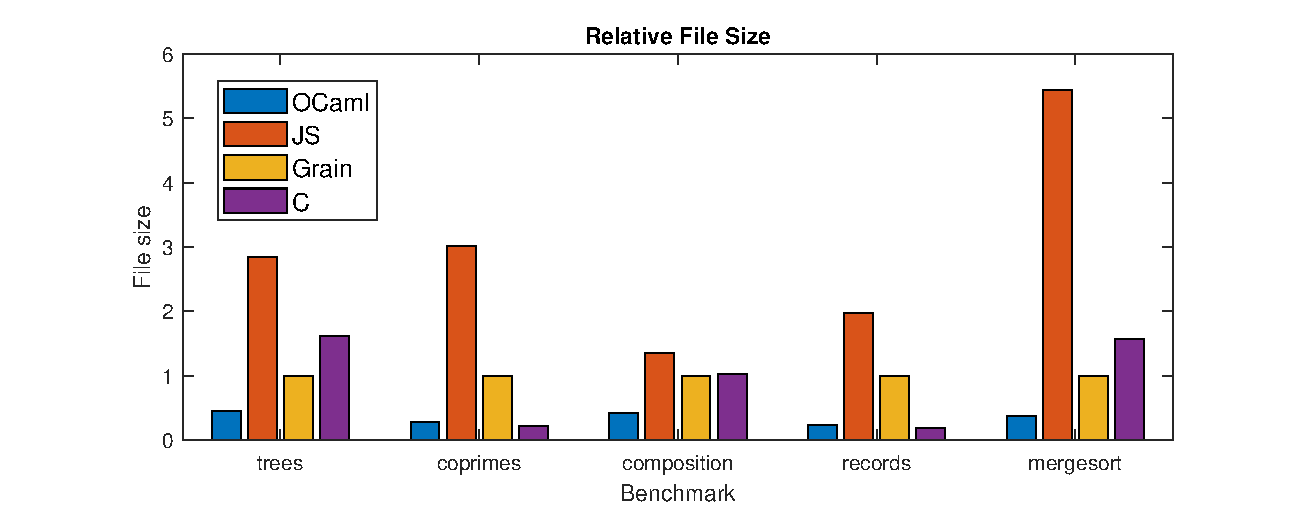
\includegraphics[scale=0.6]{filesize}
\end{figure}
\begin{itemize}
\item Measured execution time, heap usage and output file size.
\item Compiled code runs faster than both Grain and Js\_of\_ocaml output, likely due to there being no garbage collection.
\end{itemize}
\end{frame}

\begin{frame}\frametitle{Optimisations} 
\begin{itemize}
\item Tail Call Optimisation % For both functions recursive on their own and mutually recursive
\item Common Subexpression Elimination % Avoid recalculating immutable values that already exist
\item Dead Assignment Elimination % Allows compilation of pattern matching to introduce unnecessary assignments that are later removed
\end{itemize}
\text{}\\

Next task is to research garbage collection for WebAssembly.
\end{frame}


%%%%%%%%%%%%%%%%%%%%%%%%%%%%%%%%%%%%%%%%%%%%%%%%%%%%%%%%%%%%%%%%%%%%%%%%%%


%----------------------------------------------------------------------------------------

\end{document} 